\chapter{ANALISIS PERMASALAHAN DAN DESAIN SOLUSI}

\section{Analisis Permasalahan}

Standar ARINC 653 berfungsi sebagai panduan pengembangan sistem operasi \textit{real-time} pada \textit{safety-critical system}.
Banyak faktor yang menentukan apakah sebuah sistem dapat dikategorikan sebagai \textit{safety-critical system}, salah satunya adalah \textit{fault-tolerancy}.
Pada \textit{safety\hyp critical system}, \textit{fault-tolerant} adalah properti yang sangat dicari.
Sistem yang \textit{fault-tolerant} akan memberikan jaminan bahwa sistem akan terus bekerja sebagaimana seharusnya meskipun terjadi \textit{fault} selama sistem beroperasi.

Fokus dari standar ARINC 653 adalah menjamin sistem operasi melakukan partisi lingkungan eksekusi agar aplikasi yang berjalan pada sebuah lingkungan eksekusi tidak mengganggu aplikasi pada lingkungan eksekusi lainnya.
Meski standar tersebut menjamin \textit{fault} yang terjadi pada sebuah aplikasi tidak akan mengganggu aplikasi lain yang berada pada lingkungan eksekusi berbeda (\textit{fault containment}), \textit{fault} yang terjadi pada sebuah aplikasi tetap akan terjadi dan tidak ditangani.
Standar ARINC 653 mendefinisikan mekanisme untuk mendeteksi dan memberikan tanggapan apabila terjadi \textit{fault}.
Namun, standar tersebut tidak mendefinisikan tanggapan apa yang harus dilakukan untuk menjamin aplikasi yang menghasilkan \textit{fault} akan terus bekerja.
Meskipun aplikasi pada sistem tersebut akan melalui proses verifikasi untuk menjamin tidak akan terjadi \textit{fault}, proses verifikasi tersebut mungkin sangat lama atau memiliki \textit{fault} juga.
Karena itu, mekanisme penanganan \textit{fault} tidak dapat diabaikan begitu saja.

Solusi dari permasalahan tersebut adalah \textit{primary-backup scheduling}.
Penggunaan metode \textit{primary-backup scheduling} dapat menjamin bahwa aplikasi yang \textit{fault} akan tetap menjalankan \textit{backup} aplikasi tersebut yang sudah terverifikasi tidak akan mengalami \textit{fault} dalam waktu panjang.
Namun, meski sudah banyak studi mengenai \textit{primary-backup scheduling} \citep{Al-Omari2004} \citep{Bertossi2006}, belum ada studi mengenai metode tersebut spesifik pada sistem yang memenuhi standar ARINC 653.
Hal tersebut mengakibatkan sulitnya pengembangan dan verifikasi \textit{fault-tolerancy} sistem ARINC 653 yang menggunakan \textit{primary-backup scheduling}.

\section{Analisis Solusi}

Eksperimen \textit{primary-backup scheduling} akan dilakukan pada prototipe ARINC 653 pada Xen.
Hal ini dikarenakan prototipe tersebut tersedia gratis dan \textit{open-source}, sehingga pengembangan dan eksperimen yang akan dilakukan tidak memerlukan biaya banyak dan dapat dieksplorasi secara mandiri.

\subsection{Analisis Arsitektur Prototipe ARINC 653}

Prototipe ARINC 653 dibangun dengan membuat \textit{scheduler} seperti pada spesifikasi standar ARINC 653 pada Xen.
Selain itu, prototipe tersebut memberikan beberapa modul \textit{kernel} untuk menangani \textit{device} yang terpartisi sesuai dengan spesifikasi ARINC 653.
Dalam melakukan partisi memori, prototipe tersebut memanfaatkan mekanisme partisi memori menggunakan MMU yang sudah merupakan mekanisme bawaan pada Xen.

Setiap \textbf{partisi} akan direpresentasikan dengan menggunakan \textit{domain} pada Xen.
Dom0 pada Xen akan digunakan sebagai \textbf{partisi} tempat APEX dan \textit{device driver} berada, sedangkan \textbf{partisi} untuk aplikasi avionik akan direpresentasikan menggunakan domU seperti pada \autoref{figure:xen_arinc653_partitions}.

\begin{figure}[htbp]
    \centering
    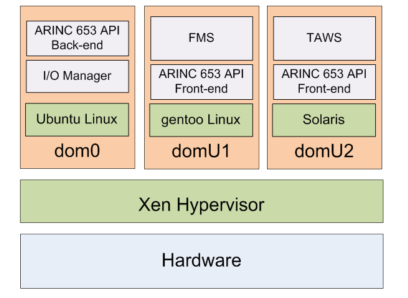
\includegraphics[scale=0.6]{resources/xen-arinc653-partitions.png}
    \caption{\textit{Hypervisor} Xen ARINC 653}
    \label{figure:xen_arinc653_partitions}
\end{figure}

\textit{Scheduling} dilakukan dengan metode seperti pada spesifikasi ARINC 653.
\textit{Task} sebuah aplikasi akan dimasukkan pada \textit{major time frame} pada saat \textit{scheduling}.
Pada Xen, hanya dom0 yang dapat memproses IRQ untuk diteruskan kepada \textit{hypervisor} atau \textit{device driver}.
Karena itu, \textit{scheduling} yang dilakukan secara berkala akan dom0 pada \textit{major time frame} seperti pada \autoref{figure:xen_arinc653_partitions_schedule}.

\begin{figure}[htbp]
    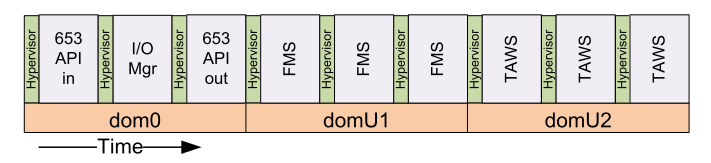
\includegraphics[scale=0.6]{resources/xen-arinc653-partition-schedule.png}
    \caption{\textit{Schedule} partisi pada Xen ARINC 653}
    \label{figure:xen_arinc653_partitions_schedule}
\end{figure}

\subsection{Implementasi \textit{Primary-Backup Scheduling} pada Prototipe ARINC 653}

Pada Xen, sebuah \textit{domain} hanya dapat dibuat oleh dom0 saja.
Aplikasi maupun \textit{scheduler} tidak dapat membuat \textit{domain} baru apabila aplikasi tersebut mengalami \textit{fault}.
Agar \textbf{partisi} \textit{backup} dapat berjalan apabila \textbf{partisi} \textit{primary} mengalami \textit{fault}, maka \textbf{partisi} \textit{backup} sudah harus dibuat oleh dom0 pada tahap inisialisasi.
\textit{Scheduler} akan memasukkan sebuah \textbf{partisi} pada \textit{major time frame} pada tahap \textit{scheduling} jika dan hanya jika \textbf{partisi} tersebut merupakan \textit{primary} dan belum mengalami kegagalan.
Jika terjadi kegagalan pada \textbf{partisi} \textit{primary}, maka \textit{scheduler} akan memasukkan \textbf{partisi} \textit{backup} yang bersesuaian pada \textit{major time frame}.
Karena itu, untuk dapat mengimplementasikan \textit{primary-backup scheduling} pada prototipe ARINC 653, \textit{scheduler} harus dapat mengetahui \textbf{partisi} mana yang merupakan \textit{primary} atau \textit{backup} agar dapat melakukan \textit{scheduling}.

Selain itu, \textit{scheduler} juga perlu mengetahui kapan sebuah \textbf{partisi} \textit{primary} dikategorikan mengalami kegagalan.
Karena itu, perlu ada mekanisme untuk mendeteksi \textit{fault}, dan memberikan informasi tersebut kepada \textit{scheduler}.

\subsubsection{Rancangan Solusi untuk Mengenali Jenis \textbf{Partisi}}

Jenis \textbf{partisi} dapat dikenali dengan menambahkan properti \textit{partition\_type} pada konfigurasi \textit{domain}, sehingga \textbf{partisi} juga mempunyai properti tersebut.
Konfigurasi \textit{domain} pada Xen dapat dilakukan dengan menggunakan \textit{xl}, salah \textit{tools} untuk melakukan manajemen \textit{domain} yang tersedia pada \textit{toolstack} milik Xen.
Fungsi untuk melakukan pengaturan dapat ditambahkan dengan memanfaatkan XAPI, yaitu \textit{interface} yang disediakan oleh Xen untuk menambahkan fungsionalitas.
Fungsionalitas yang akan ditambahkan adalah fungsionalitas untuk mendefinisikan \textit{partition\_type} pada \textit{xl}.
\textit{Scheduler} akan dapat mendeteksi jenis \textit{domain} melalui informasi tersebut.

\subsubsection{Rancangan Solusi untuk Mendeteksi Kegagalan}

Pada Xen, sebuah dom0 dapat mendefinisikan aksi yang harus dilakukan apabila sebuah \textit{domain} mengalami \textit{crash}.
Salah satu aksi yang dapat dilakukan adalah menghapus \textit{domain} tersebut, sehingga permasalahan apabila kegagalan yang dialami adalah \textit{crash}, \textit{domain} tersebut otomatis tidak akan diberikan pada \textit{scheduler}.
Namun, apabila permasalahan yang terjadi adalah \textit{deadline} yang tidak terpenuhi, atau kesalahan yang tidak mengakibatkan \textit{crash}, maka aplikasi harus mengirim IRQ kepada \textit{hypervisor}.
IRQ yang diberikan akan ditangani melalui dom0 yang dapat mengatur \textit{domain}, sehingga IRQ tersebut dapat menjadi pertanda bahwa \textit{domain} yang mengirimkan IRQ tersebut mengalami kegagalan dan meminta dom0 untuk menanganinya.
Berikut beberapa penanganan yang dapat dilakukan oleh dom0:
\begin{itemize}
    \item Menghapus \textit{domain} yang mengirim IRQ tersebut
    \item Mengganti properti \textit{domain} menjadi \textit{temporary-primary}
\end{itemize}
Pemilihan penanganan akan ditentukan setelah studi lebih lanjut.

\subsection{Pengujian dan Pengambilan Hasil}

Pengujian \textit{real-time} akan dilakukan dengan melakukan \textit{stress-testing} menggunakan \textit{scheduler} tertentu.
\textit{Scheduler} yang akan diuji adalah \textit{scheduler} bawaan prototipe ARINC 653 dan \textit{scheduler} implementasi \textit{primary-backup scheduling}.
\textit{Stress-testing} dilakukan dengan menggunakan aplikasi yang akan menjalankan sebuah proses subjek dan menjalankan beberapa proses \textit{background} (mungkin nol).
Proses subjek akan memberikan laporan secara berkala pada aplikasi penguji apakah \textit{deadline} dari \textit{task} yang dibutuhkan terpenuhi atau tidak.

Pengujian \textit{fault-tolerancy} akan dilakukan dengan melakukan \textit{question-answering} antara aplikasi dengan proses subjek.
\textit{Question-answering} dilakukan sebagai berikut:
\begin{enumerate}
    \item Aplikasi pengujian akan meminta proses subjek untuk menghitung suatu nilai berdasarkan input tertentu (misal menghitung nilai $sqrt{n}$).
    \item Proses subjek akan mengambil nilai semi-acak, berdasarkan nilai tersebut proses dapat melakukan salah satu dari:
        \begin{itemize}
            \item Proses subjek akan menghitung nilai tersebut dan memberikan
            \item Proses subjek akan mengakitvasikan mekanisme \textit{fault detection}.
        \end{itemize}
    \item Aplikasi pengujian akan melakukan validasi kebenaran hasil perhitungan
\end{enumerate}
Untuk pengujian ini, aplikasi pengujian tidak akan menjalankan proses \textit{background} sama sekali.

Kedua metode ini akan memberikan persentase \textit{real-time} serta \textit{fault-tolerancy} \textit{scheduler} yang digunakan pada saat pengujian.
Nilai semi-acak yang akan digunakan sebagai ambang batas keputusan proses subjek akan ditentukan sedemikian sehingga memiliki \textit{mean time to failure} yang diharapkan.
Hasil pengujian akan memberikan statistik faktor-faktor yang penting untuk sebuah \textit{scheduler}.

% vim: wrap
